\documentclass[a4paper,12pt, oneside]{article}
\usepackage{geometry} 
\geometry{letterpaper}
\usepackage[parfill]{parskip}
\usepackage{graphicx}
\usepackage{amssymb}
\usepackage{amsmath}
\usepackage[usenames, dvipsnames]{color}
\usepackage[margin=1.5cm]{caption}
\usepackage{subcaption}
\usepackage [english]{babel}
\usepackage [autostyle, english = american]{csquotes}
\usepackage{float}
\usepackage{verbatim}
\usepackage[normalem]{ulem}
\usepackage{siunitx}
\usepackage{url}

\usepackage{array}
\newcolumntype{L}[1]{>{\raggedright\let\newline\\\arraybackslash\hspace{0pt}}m{#1}}
\newcolumntype{C}[1]{>{\centering\let\newline\\\arraybackslash\hspace{0pt}}m{#1}}
\newcolumntype{R}[1]{>{\raggedleft\let\newline\\\arraybackslash\hspace{0pt}}m{#1}}

\MakeOuterQuote{"}

\newcommand{\red}[1]{\textcolor{red}{#1}}
\newcommand{\blue}[1]{\textcolor{blue}{#1}}
\newcommand{\green}[1]{\textcolor{green}{#1}}

\usepackage{mathtools}
\newcommand\givenbase[1][]{\:#1\lvert\:}
\let\given\givenbase
\newcommand\sgiven{\givenbase[\delimsize]}
\DeclarePairedDelimiterX\Basics[1](){\let\given\sgiven #1}
\newcommand\Average{E\Basics}

\newcommand*{\myinfinity}{{\propto}}

\title{Constraining Frisbee Tracking Methods Through Bayesian Analysis of Flying Disc Models}
\author{Lizzie Hannah}
\date{\today}

\begin{document}
\maketitle

\section{Introduction}

Flying discs have long provided a source of entertainment for dogs and humans alike.  The modern Frisbee -- first produced by Wham-O Inc. toy company in 1957 -- is today a staple in household toy boxes across the United States.  While the precise details of the Frisbee's history continue to be a source of debate, experts generally credit Civil War era baker William Russel Frisbie with designing the baking tin that ultimately became the first Frisbee prototype.  Yale University students purchased Frisbie's pies and played catch by tossing their empty tins around; thus the idea for the Frisbee was borne \cite{frisorigins}.  

In the late 1940s, Walter Frederick Morrison designed and manufactured the first plastic disc, eventually partnering with Wham-O for mass production and marketing \cite{frisorigins}. Since then, flying discs have exploded in popularity, providing the basis for sports like Ultimate Frisbee and disc golf. Ultimate Frisbee, a game that combines elements of football and soccer into a fast-paced field sport, is estimated to be played by 7 million people around the globe \cite{frisstats}.  Disc golf (as the name suggests) bears many similarities to standard golf: disc golfers compete by throwing discs from "tees" towards targets, aiming to reach the target with as few throws as possible. Though disc sports are relatively young, they are slowly gaining widespread acceptance in the arena of competitive athletics. Indeed, in 2015 the International Olympics Committee granted full recognition to the World Flying Disc Federation, indicating that disc sports may appear in future Olypmic Games \cite{iocrecognition}.

While Wham-O continues to hold a trademark on the term "Frisbee," numerous companies (including Discraft, Innova, EuroDisc, and others) have emerged as competitors in the flying disc market. It is worth mentioning here that, while all flying discs retain the same basic shape, it is possible to observe subtle differences in the trajectories of their flights.  A thick, heavy discus, for example, flies along an entirely different trajectory than a small, light clay pigeon, which in turn travels in a manner distinct from that of a standard Frisbee \cite{pottsandcrowther2007}. As disc sports become increasingly competitive, it will be in the best interest of athletes, coaches, and fans to better understand the aerodynamics of of flying discs.

\red{[Pics of discus, Frisbee, and clay pigeon]}

Despite the recent growth of disc sports, the current body of Frisbee research remains relatively limited. Previous research has developed physics-based models of flying discs, but these models have yet to be refined such that they can predict the flight trajectory of any disc given any set of initial conditions \cite{H3, pottsandcrowther2007, yasuda, mitchell, stilleyandcarstens, morrison}. In particular, the accuracy of the existing models depends heavily on the accuracy of experimental flight data, which is difficult to obtain with without expensive equipment and sophisticated tracking software \cite{H3}.

Understanding the dynamics of Frisbee flight may enable athletes and coaches to improve their performance in sports like Ultimate Frisbee and disc golf.  More generally, however, spinning flying objects display unique and interesting aerodynamic properties, governed by the same principles that guide sophisticated flying vehicles and spacecraft \cite{lorenz2004}. Simply put, a Frisbee is a combination of a wing and a gyroscope. Thus, Bernoulli's Principle (which controls the motion of wings) provides the lift that keeps a Frisbee in the air during flight, and the spin of a Frisbee provides the gyroscopic stability required for a flying disc to maintain its directionality \cite{morrison}. Because of their size and accessibility, Frisbees are convenient objects on which to study patterns of flight in a lab setting. Thus, developing accurate and reliable models of Frisbee throws may prove relevant in designing more complex flying objects. 
 
The basis for the work presented hereafter is \textit{Frisbee Flight Simulation and Throw Biomechanics}, published by as a master's thesis by Sarah Hummel in 2003 and subsequently denoted H3. H3 provides a highly comprehensive review of currently available Frisbee literature and builds on the work of (among others) Potts \& Crowther, Yasuda, Mitchell, and Stilley \& Carstens \cite{H3, pottsandcrowther2007, yasuda, mitchell, stilleyandcarstens}. 

Ultimately, the goals of this Honors Thesis are twofold. The first goal is to reproduce the model described in H3 using a format that is accessible to a relatively wide, general audience, and the second is to compare the model against data using Bayesian analysis. We will use this analysis to begin understanding how video tracking methods can be used to capture the trajectories of flying discs. Past work has captured Frisbee flight data by attaching accelerometers and gyroscopes to flying discs, but such electronic devices have the potential to alter a disc's true trajectory \cite{lorenz2004}. Video tracking methods, which do not affect the movement of flying objects, may prove to be more reliable and efficient than electronic tracking methods, but only if the cameras used for data capture are of sufficient quality. To effectively employ video tracking methods, it will be important to establish threshold values for intrinsic properties of cameras, such as frames per second (FPS), that generate meaningful sets of data. This Honors Thesis will begin investigating the relationship between FPS and data precision, which will aid future researchers in setting more exact constraints on cameras used to capture Frisbee flight data. 

\section{Frisbee Model}

\subsection{Forces}
Understanding the forces that act upon a disc during flight is essential to modeling the trajectory of a Frisbee throw. Three primary forces influence the translational motion of a flying disc: lift, drag, and gravity. Gravity, of course, points vertically downward from the Frisbee's center of mass.  The drag force points in the direction opposite the disc's velocity, working to slow down the Frisbee, and the lift force acts in the direction perpendicular to drag \cite{H3}. The total force acting on a Frisbee is the sum of all the forces.
\begin{figure}[h]
        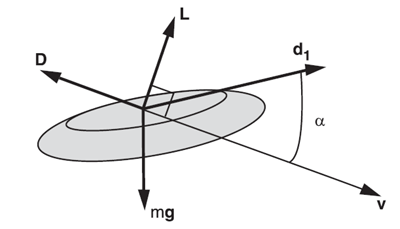
\includegraphics[width=6cm, height=4cm]{frisforces}
	\centering
	\caption{Diagram of forces acting on Frisbee. Note that $\alpha$ denotes angle of attack, the angle between the plane of the disc and the disc's velocity. Figure from Hubbard \& Hummel, 2000. \cite{hubbardandhummel}}
	\label{fig:discforces1}
\end{figure}
To calculate the magnitude of the gravitational force acting on a Frisbee, we simply multiply the mass of a standard Frisbee (0.175 kg) by the constant of gravitational acceleration, here defined as  9.81 $m/s^{2}.$ 
 
The calculation of the lift and drag forces acting on a flying disc, though slightly more complicated than the calculation of the gravitational force, is completed in a similarly standard way. In general, we define the lift and drag forces in terms of two coefficients, $C_L$ and $C_D$, respectively, that in turn depend on various quantities \cite{H3}. The magnitudes of the lift and drag forces (denoted $F_L$ and $F_D$) are given by the following equations:

\begin{equation}
  F_D=C_DAv^2\rho/2,
\end{equation}
\begin{equation}
  F_L=C_LAv^2\rho/2
\end{equation}

where \textit{A} is the area of a standard disc (0.057 $m^2$), \textit{v} is the velocity of a thrown disc at time \textit{t}, and $\rho$ is the density of air (taken here to be the average value at sea level of 1.225 $kg/m^3$). 

For the purposes of our work, both $C_L$ and $C_D$ are solely functions of $\alpha$, the angle of attack, defined as the angle between the disc's velocity and the plane of the disc (Figure \ref{fig:discforces1}). In reality, $C_D$ also depends on a disc's Reynolds number and an angular velocity-dependent spin parameter, and $C_L$ depends on the air pressure above and below the Frisbee. These factors, however, are either a) negligible in calculating the overall trajectory of a flying disc or b) highly complex and beyond the scope of this analysis \cite{H3}. Thus, only $\alpha$ is included here.

The lift and drag coefficients further depend on a series of parameters that are specific to individual discs (or types of discs); these parameters are constant values that serve to distinguish the trajectory of one Frisbee throw from that of another \cite{hubbardandhummel}.  The drag coefficient has quadratic dependence on $\alpha$, and the lift coefficient has linear dependence on $\alpha$. We will use $\alpha_0$ to denote the value of $\alpha$ at which $F_D$ is at a minimum and $F_L=0$ , here assumed to be $-4^{\circ}$ \cite{H3}. (At $-4^{\circ}$ the front of the disc is tilted at a slight downward angle.) 

\begin{equation}
  C_D=P_{D0}+P_{D\alpha}(\alpha-\alpha_0)^2
\end{equation}
\begin{equation}
  C_L=P_{L0}+P_{L\alpha}\alpha
\end{equation}
\begin{figure}[H]
	\centering
	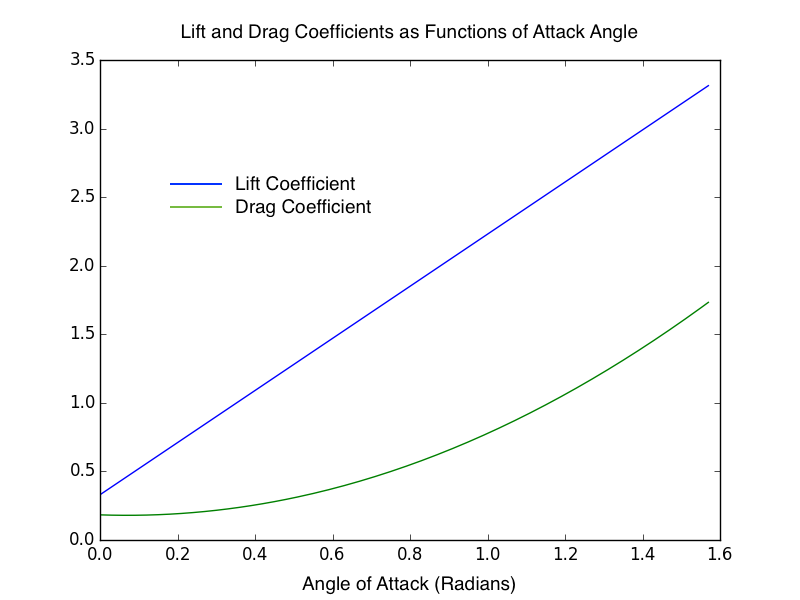
\includegraphics[width=10cm, height=7.5cm]{liftanddrag}
	\caption{Lift and drag coefficient values as functions of $\alpha.$ Plotted for $\alpha$ ranging from 0 to $\frac{\pi}{2}$.}
\end{figure}
It is these parameters ($P_{D0}, P_{D\alpha}, P_{L0}$, and $P_{L\alpha}$) that form the crux of this Honors Thesis. Previous research has attempted to calculate $P_{D0}, P_{D\alpha}, P_{L0}$, and $P_{L\alpha}$ for a standard 0.175 kg Discraft Ultrastar disc (Table 1), but to date no consensus on their values exists among the literature \cite{H3, pottsandcrowther2007, yasuda, stilleyandcarstens}. The work presented here will offer a parameter estimation method that can be applied to future studies.

\begin{table}[h]\label{tab:1}
\centering
\begin{tabular}{| c | c | c | c | c |}
\hline
$\bf{Author}$ & $\bf{P_{L0}}$ & $\bf{P_{L\alpha}}$ & $\bf{P_{D0}}$ & $\bf{P_{D\alpha}}$ \\ \hline
H3 & 0.33 & 1.91 & 0.18 & 0.69  \\ \hline
Potts \& Crowther & 0.2 & 2.96 & 0.08 & 2.72 \\ \hline
Yasuda & 0.08 & 2.4 & 0.1 & 2.3 \\ \hline
Stilley \& Carstens & 0.15 & 2.8 & 0.1 & 2.5 \\ \hline
\end{tabular}
\caption{Top line is parameter values reported in H3. All table values previously reported in H3 and calculated by authors in leftmost column.}
\end{table} 

Note that model presented here generally ignores environmental factors (like wind and rain) that might affect a disc's flightpath, and they further ignore factors such as airflow that could only be accounted for using fluid dynamics. Instead, the forces and torques outlined here appeal to solely classical mechanics in their description of a Frisbee's motion.
\subsection{Torques}

In order to produce a representative model of a Frisbee flight in three dimensions, we must consider the torques that cause the disc to rotate about each of its axes. As with the lift and drag forces, the magnitudes of the torques in the \textit{x}, \textit{y}, and \textit{z} directions are calculated using three standard equations that depend on a series of parameters (described by H3 and references therein). Here we will use $\tau$ to denote torque.\begin{comment} and we will define $\phi$ to be the angle about the \textit{x}-axis, $\theta$ to be the angle about the \textit{y}-axis, and $\gamma$ to be the angle about the \textit{z}-axis.
\begin{figure}[H]
	\centering
	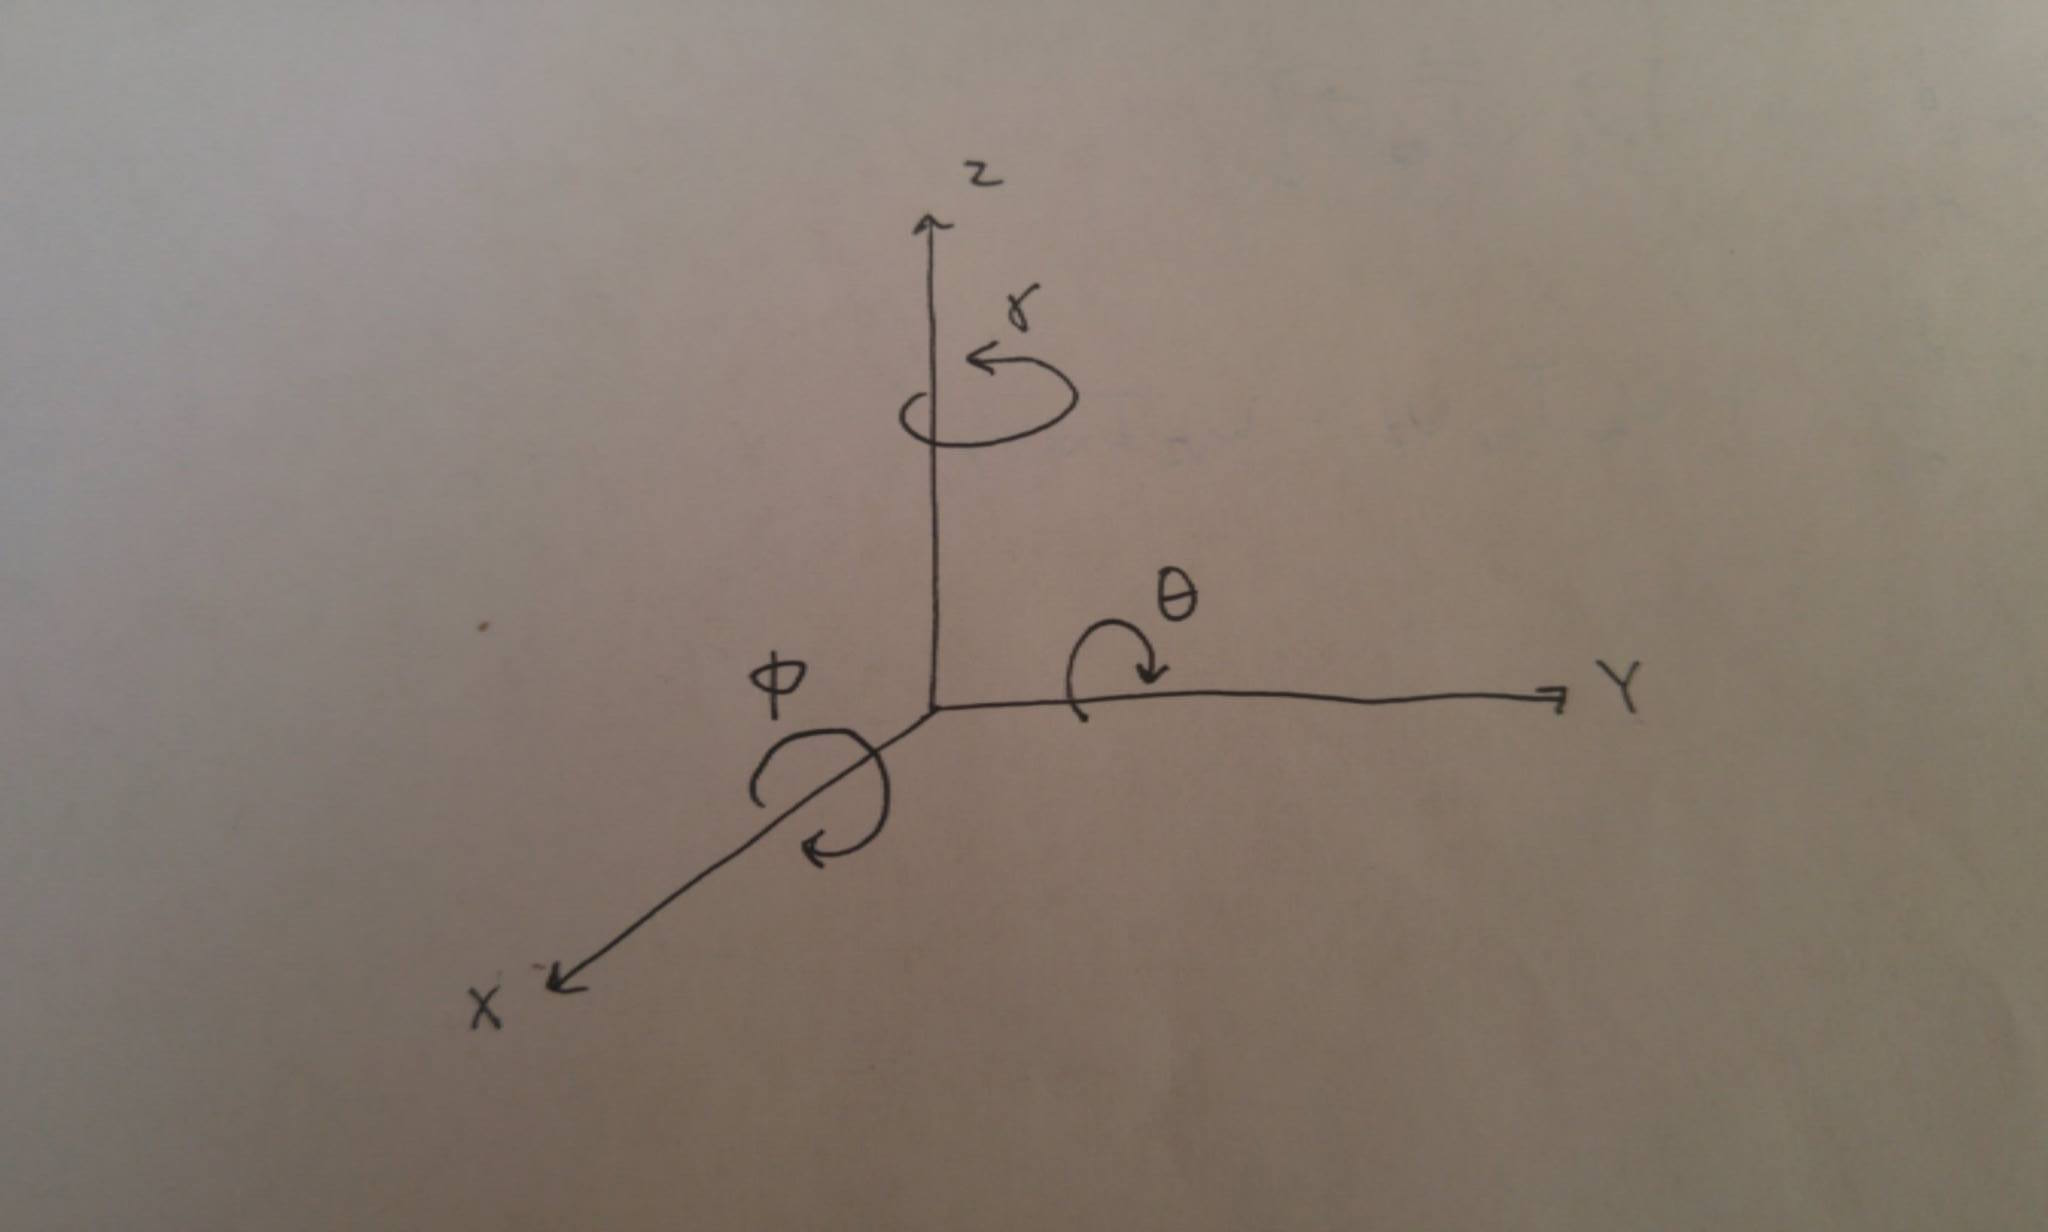
\includegraphics[width=10cm, height=6cm]{AxesDiagram}
	\caption{\red{Fix and make prettier, obvi}}
\end{figure}
\end{comment}

The magnitude of the torque around the \textit{x}-axis depends on two parameters, $P_{\tau_x\omega_x}$ and $P_{\tau_x\omega_z}$, which are multiplied by $\omega_x$ and $\omega_z$, respectively. From here on, $\omega$ denotes angular velocity. From standard classical mechanics,
\begin{equation}
  \tau_x=(P_{\tau_x\omega_x}\omega_x+P_{\tau_x\omega_z}\omega_z)\frac{1}2Av^2d.
\end{equation}
As before, \textit{A} is the area of a standard disc in m$^2$, \textit{v} is the disc's velocity at time \textit{t}, and \textit{d} is the diameter of a standard disc, here taken to be $\sqrt\frac{1.14}\pi$ m.

Similarly $\tau_y$ and $\tau_z$ are written as,
\begin{equation}
  \tau_y=(P_{\tau_{y0}}+P_{\tau_y\omega_y}\omega_y+P_{\tau_{y\alpha}}\alpha)\frac{1}2Av^2d
\end{equation}
\begin{equation}
  \tau_z=(P_{\tau_z\omega_z}\omega_z)\frac{1}2Av^2d.
\end{equation}

Although the torque parameters described above are critically important to the flight dynamics of Frisbees, this Honors Thesis will not examine them in great detail. Instead, we will focus here on the lift and drag parameters, choosing to simplify our analysis by concentrating solely on $P_{D0}, P_{D\alpha}, P_{L0}$, and $P_{L\alpha}$. The torque parameters will be fixed at the values reported in Table 1. A truly comprehensive analysis of flying disc trajectories should expand the work described here to include the torque functions.

\subsection{Newton's Equations of Motion} 

According to classical mechanics, the motion of rigid bodies can be described by two of Newton's equations, which relate an object's translational and rotational trajectory to the sum of the forces and torques acting upon it (7).  The Newton-Euler equations of motion are derived from Newton's two laws of motion for rigid bodies:
\begin{equation}
  \label{eq:newton1}
  \vec{F}=\textit{m}\vec{a}
\end{equation}
\begin{equation}
  \label{eq:newton2}
  \vec{M}=\dfrac{\vec{dL}}{dt}
\end{equation}
Equation \ref{eq:newton1} states that the sum of the forces acting upon a rigid body is equal to the product of the body's mass $\textit{m}$ and its acceleration $\vec{a}$, where $\vec{a}$ is simply a time derivative of the body's velocity.  

Equation \ref{eq:newton2} states that a rigid body's angular momentum $(\vec{dL}/dt)$ changes at a rate equal to the sum of the torques $(\vec{M})$ acting upon it. Here we have $\vec{L}$=\textit{I}$\vec{w}$, where \textit{I} is the mass moment of inertia matrix and $\vec{w}$ is the body's angular velocity vector. Due to the axial symmetry of a disc, the inertial matrix for a Frisbee is defined as,  
\begin{equation*}
I=\begin{bmatrix}
I_{xx} & 0 & 0 \\
0 & I_{yy} & 0 \\ 
0 & 0 & I_{zz}
\end{bmatrix},
\end{equation*}
where $I_{xx}$=$I_{yy}=0.00122$ and $I_{zz}=0.00235$ is distinct \cite{hubbardandhummel}.  The nature of $\vec{w}$ depends on a series of rotations that rotate the Frisbee between a standard \textit{xyz} coordinate axis to a new axis, here denoted \textit{x'y'z'} \cite{H3}. These rotations are discussed in the following sections.

\subsection{Euler Rotations} 
%Useful info: https://en.wikipedia.org/wiki/Rotating_reference_frame
%Useful info: https://en.wikipedia.org/wiki/Euler_force
H3's Frisbee model takes into account several reference frames, which are coordinate systems that describe an object's orientation.  In the following discussion, the term "lab frame" refers to an inertial reference frame specified by Cartesian coordinates $x,y,z$, where the \textit{xy} plane is horizontal and the positive \textit{z} axis points upward.  (Note that H3 defines the +\textit{z} direction to be down, while here we define it to be up.) The term "Frisbee frame" refers to a body-fixed coordinate system, \textit{x', y', z'}, in which the \textit{x'y'} plane lies on top of -- or parallel to -- the plane of the Frisbee. 

We rotate the coordinates of a disc from the \textit{x,y,z} lab frame to the \textit{x',y',z',} Frisbee frame by performing a series of matrix rotations about intermediate sets of axes.  The rotations used here are those described in H3, which rotate the Frisbee as follows: 1) about the \textit{x}-axis through angle $\phi$ into an intermediate set of axes denoted $\chi,\eta,\zeta$, 2) about the $\eta$-axis through angle $\theta$ into an intermediate set of axes denoted $\chi',\eta',\zeta'$, and 3) about the $\zeta'$ axis through angle $\gamma$ into \textit{x', y', z'}.

Rotations 1-3 are achieved with three rotation matrices, which can be multiplied together to form a single comprehensive rotation matrix. Rotation 1 can be expressed by the matrix,
\begin{equation*}
C(\phi)=\begin{bmatrix}
1 & 0 & 0 \\
0 & \cos\phi & \sin\phi \\
0 & -\sin\phi & \cos\phi
\end{bmatrix}.
\end{equation*}

Rotation 2 can be expressed by the matrix, 
\begin{equation*}
B(\theta)=\begin{bmatrix}
\cos\theta & 0 & -\sin\theta \\
0 & 1 & 0 \\
\sin\theta & 0 & \cos\theta
\end{bmatrix}.
\end{equation*}

Rotation 3 can be expressed by the matrix, 
\begin{equation*}
D(\gamma)=\begin{bmatrix}
\cos\gamma & \sin\gamma & 0 \\
-\sin\gamma & \cos\gamma & 0 \\
0 & 0 & 1
\end{bmatrix}.
\end{equation*}

In general, we would express the final Euler rotation matrix as a product of B, C, and D. However, for the purposes of modeling a Frisbee trajectory, we have chosen to rotate the original $x, y, z$ axes only onto the plane of the disc, not onto the spinning disc. This choice was made for the sake of simplifying the model and the numerical calculations it requires \cite{H3}. Rotating the $x, y, z$ axis onto the plane of the disc only requires rotations 1 and 2, which rotate through $\phi$ and $\theta$, respectively.

Therefore, the complete rotation matrix, which we use to rotate the Frisbee's coordinates from the inertial lab frame into the Frisbee frame, is described as follows:

\begin{equation*}
A(\phi,\theta,\gamma)=A(\phi,\theta)=B(\theta)C(\phi)=\begin{bmatrix}
\cos\theta & \sin\phi\sin\theta & -\sin\theta\cos\phi \\
0 & \cos\phi & \sin\phi \\
\sin\theta & -\sin\phi\cos\theta & \cos\phi\cos\theta
\end{bmatrix}.
\end{equation*}

\subsection{Angular Velocities}

We can denote the angular velocities of the Frisbee as $\vec{w}_\phi$, $\vec{w}_\theta$, and $\vec{w}_\gamma$.  According to Goldstein, Poole, \& Safko, these angular velocities point along the "axes that their angles are rotated about" \cite{gps}.

Consider, for example, $\vec{w}_\phi$.  Before performing any rotations, the vector $(\dot\phi, 0, 0)$ points along the original \textit{x}-axis.  The original \textit{x}-axis is ultimately rotated through angles $\phi$ and $\theta$ via matrices C and B, as described above. In other words, the original \textit{x}-axis undergoes a full transformation by the matrix A$(\phi,\theta)$. Therefore, in order to determine the direction of $\vec{w}_\phi$, we must rotate $(\dot\phi, 0, 0)$ about angles $\phi$ and $\theta$.  This rotation yields:

\begin{equation*}
\vec{w}_\phi=A(\phi,\theta)\left(\begin{array}{ccc}\dot\phi\\0\\0\end{array} \right)=\left(\begin{array}{ccc}\dot\phi\cos\theta\\0\\\dot\phi\sin\theta\end{array} \right).
\end{equation*}

Similarly, in order to find $\vec{w}_\theta$ and $\vec{w}_\gamma$, we can rotate $(0, \dot\theta, 0)$ and $(0, 0, \dot\gamma)$ about the angles through which their original axes are rotated. The vector $(0, \dot\theta, 0)$ originally points along the intermediate $\eta$ axis, which only rotates through the angle $\theta$. As such, we have:
\begin{equation*}
  \vec{w}_\theta=B(\theta)\left(\begin{array}{ccc}
    0\\
    \dot\theta \\
    0
  \end{array} 
  \right)=\left(\begin{array}{ccc}
    0 \\ 
    \dot\theta \\
    0
  \end{array}\right).
\end{equation*}

Since we have only chosen to rotate the original axes of the Frisbee onto the plane of the disc (ignoring spin), the rate at which the angles in the Frisbee frame are changing is equal to the sum $\vec{w}_\phi+\vec{w}_\theta$. Thus,
\begin{equation*}
\vec{w}_F=\left(\begin{array}{ccc}\dot\phi\cos\theta\\\dot\theta\\\dot\phi\sin\theta\end{array} \right)
\end{equation*}

The angular velocity of the Frisbee itself accounts for the final component, $\vec{w}_\gamma$, which already lies along the \textit{z'}-axis after undergoing rotations through $\phi$ and $\theta$. This means that the vector $(0, 0, \dot\gamma)$ does not require any additional rotations, and 
\begin{equation*}
\vec{w}_{Total}=\vec{w}_\gamma+\vec{w}_F=\left(\begin{array}{ccc}\dot\phi\cos\theta\\\dot\theta\\\dot\phi\sin\theta+\dot\gamma\end{array} \right)
\end{equation*}

\subsection{Second-Order Equations}

Ultimately, grouping Euler's laws of motion together in terms of vectors and matrices yields the Newton-Euler equations of motion (expressed below), which are assumed to govern the flight paths of Frisbees (H3). 
\begin{equation}
  \label{eq:newton3}
  \vec{F}=\textit{m}(\dfrac{\vec{dv}}{dt}+\vec{\textit{w}}_F\times\vec{v})
\end{equation}
\begin{equation}
  \label{eq:newton4}
  \vec{M}=I\dfrac{\vec{dw}}{dt}+\vec{\textit{w}}_F\times I \vec{w}
\end{equation}

Since we have already written explicit equations for $\textit{w}_F$ and $\textit{w}_{Total}$, we can write the righthand side of Equations 9 and 10 in terms of $\phi$, $\theta$, and $\gamma$. In doing so, we can derive ordinary differential equations (ODEs) that describe both the translational and angular accelerations of a Frisbee throughout its flight. These second-order ODEs can be transformed into a system of first-order ODEs, which can be numerically integrated in order to determine the position and velocity of a disc at any time during its trajectory. 

%\blue{STOP! YOU HAVE MIXED NOTATION FOR TIME DERIVATIVES!! You use dot notation $(\dot{\theta})$ in the section above, and you use dash notation $(\theta')$ below. This is difficult to read because these derivaives have different meanings to physicists. Everything should be dot notation. Fix this.}

First, we calculate $\vec{w}_F\times\vec{v}$: 
\begin{equation*}
\vec{w}_F\times\vec{v}=\left(\begin{array}{ccc} v_z\dot\theta-v_y(\dot\gamma+\dot\phi\sin\theta) \\ v_x(\dot\gamma+\dot\phi\sin\theta)-v_z\dot\phi\cos\theta \\ v_y\dot\phi\cos\theta-v_x\dot\theta\end{array}\right).
\end{equation*}

Substituting $\vec{w}_F\times\vec{v}$ into (9), we can solve for acceleration. Thus,

\begin{equation}
\frac{{dv}_x}{dt}=\frac{{F}_x-\dot\theta v_z+v_y(\dot\phi\sin\theta)}{m}
\end{equation}

\begin{equation}
\frac{{dv}_y}{dt}=\frac{F_y-v_x\dot\phi\sin\dot\theta+v_z\dot\phi\cos\theta}{m}
\end{equation}

\begin{equation}
\frac{{dv}_z}{dt}=\frac{F_z-v_y\dot\phi\cos\theta+v_x\dot\theta}{m}
\end{equation}

Next, to solve for angular acceleration, we observe that 
\begin{equation}
  \label{eq:dwdt}
\frac{\vec{dw}}{dt}=\left(\begin{array}{ccc}\ddot\phi\cos\theta-\dot\phi\dot\theta\sin\theta\\ \ddot\theta \\ \ddot\phi\sin\theta + \dot\phi\dot\theta\cos\theta+\ddot\gamma\end{array} \right)
\end{equation}

Substituting (\ref{eq:dwdt}) into (10) and solving for $\ddot\phi$, $\ddot\theta$, and $\ddot\gamma$ yields,
\begin{equation}
\ddot\phi=\frac{M_x-I_{zz}\dot\theta(\dot\phi\sin\theta+\dot\gamma)+2I_{xx}\dot\phi\dot\theta\sin\theta}{I_{xx}\cos\theta}
\end{equation}

\begin{equation}
\ddot\theta=\frac{M_y+I_{zz}\dot\phi\cos\theta(\dot\phi\sin\theta+\dot\gamma)-I_{yy}\dot\phi^2\sin\theta\cos\theta} {I_{yy}}
\end{equation}

\begin{equation}
\ddot\gamma=\frac{M_z-I_{zz}(\dot\phi\dot\theta\cos\theta-\ddot\phi\sin\theta)}{I_{zz}}
\end{equation}

At this point, we have a system of second-order ODEs. Equations 12-14 calculate the translational acceleration of a disc in each direction at time \textit{t}, and Equations 16-18 calculate the angular acceleration of a disc at time \textit{t}.

\subsection{Position Coordinates}
 %\blue{You have hard coded ``equations 12-17'', but the numbers have changed. Learn to use the ref\{\} and label\{\} tools.}
Our goal is to use equations 12-14 and 16-18 to determine the positional coordinates of a Frisbee over the course of its trajectory. Letting $\vec{r}=$ denote the \textit{x, y}, and \textit{z} Euclidean positions of a disc during its flight, then 

\begin{equation}
  \label{eq:position_deriv}
  \frac{d\vec{r}}{dt} = \vec{v}.
\end{equation}

Similarly, letting $\phi, \theta$, and $\gamma$ denote the Euler angles of the disc, then
\begin{equation}
\frac{d\phi}{dt}=\dot\phi
\end{equation}
\begin{equation}
\frac{d\theta}{dt}=\dot\theta
\end{equation}
\begin{equation}
\frac{d\gamma}{dt}=\dot\gamma.
\end{equation}
where we obtain $\dot\phi, \dot\theta$, and $\dot\gamma$ via numerical integration of $\ddot\phi, \ddot\theta$, and $\ddot\gamma$. Likewise, we obtain the components of $\vec{r}$ via numerical integration of $\frac{{dv}_x}{dt}, \frac{{dv}_y}{dt}$, and $\frac{{dv}_z}{dt}$. It follows, then, that by integrating equations 19-22 over time $t_0$ to $t_f$, we can obtain the Euclidean positions and Euler angles of Frisbee, allowing us to simulate the flight coordinates of a flying disc. 

\section{Parameter Estimation}
\subsection{Bayes' Theorem}
Bayes' theorem states:
\begin{equation}
\bold{P}(\theta\given\bold{X})=\frac{\bold{P(\theta})\cdot\bold{P({X}\given\theta})}{\bold{P(\bold{X})}},
\end{equation}
where $\theta$ denotes a set of unknown parameters and $\bold{X}$ denotes a known data set. Here, $\theta$ is a vector that contains  $P_{D0}, P_{D\alpha}, P_{L0}$, and $P_{L\alpha}$, and $\bold{X}$ denotes a data set obtained from a simulated Frisbee throw, including time, position, and velocity coordinates. These coordinates were produced from our Frisbee model, which generated a trajectory using the specified parameter values shown below.
\begin{table}[h]\label{tab:2}
\centering
\begin{tabular}{| C{2.5cm} | C{2.5cm} | C{2.5cm} | C{2.5cm} | C{2.5cm} |}
\hline
$P_{L0}$ & $P_{L\alpha}$ & $P_{D0}$ & $P_{D\alpha}$  &  $P_{\tau_{x,\omega_x}}$ \\ \hline
0.33 & 1.9 & 0.18 & 0.69 & 0.43 \\ \hline
\end{tabular}
\begin{tabular}{| C{2.5cm} | C{2.5cm} | C{2.5cm} | C{2.5cm} | C{2.5cm} |}
\hline
$P_{\tau_{x,\omega_z}}$  & $P_{\tau_{y0}}$ & $P_{\tau_{y\alpha }}$ & $P_{\tau_{y,\omega_y}}$ & $P_{\tau_{z,\omega z }}$\\ \hline
\num{-1.4e-2} & \num{-8.2e-2} & \num{-1.2e-2} & \num{-1.7e-3} & \num{-3.4e-5} \\ \hline
\end{tabular}
\caption{Parameter values (reported in H3) used to generate simulated data set.}
\end{table}

The conditional probability $\bold{P(\theta\given\bold{X})}$ is the posterior probability distribution of $\bold{\theta}$ given $\bold{X}$. This term denotes the probability of observing a certain set of parameters given specific set of data (i.e. coordinate points generated from an actual Frisbee throw). $\bold{P({X}\given\theta})$, in contrast, gives the likelihood of observing given data set conditional on certain parameters. For example, if we know that $P_{D0}=0.1, P_{D\alpha}=0.2, P_{L0}=0.3$, and $P_{L\alpha}=0.4$, we can calculate the probability that each element in $\bold{X}$ takes a certain value.  $\bold{P(\theta)}$ is known as the prior, which describes any knowledge about $\theta$ that exists in the absence of details regarding $\bold{X}$. This prior might incorporate, for instance, physical constraints on a flying object, such as the impossibility of observing negative z-values. In our setting, negative z-values would indicate that a flying disc continued moving downward after hitting the ground.

$\bold{P(\bold{X})}$ expresses the likelihood of our known data set $\bold{X}$. In practice we will ignore this term because we cannot determine the likelihood of $\bold{X}$ ahead of time without empirical evidence. To put it another way, we impose a normalization that doesn't depend on our model at all. Thus, rewriting Bayes' theorem in terms of natural logarithms, we have,
\begin{equation}
\ln\bold{P}(\theta\given\bold{X})=\ln{\bold{P(\theta})+\ln\bold{P({X}\given\theta})}.
\end{equation}

Equation 24 will be used to assess our Frisbee model.  Specifically, we will use Markov chain Monte Carlo analysis to sample the posterior probability distribution function of each of the four parameters. 


\subsection{Prior Function}
We begin our analysis by defining a prior function $\bold{P(\theta)}$ that is relevant to our simulated Frisbee throw. In general, this prior function should account for knowledge from past research and physically impossible conditions. However, given the lack of literature surrounding the trajectories of flying discs, such information cannot accurately be incorporated into our analysis.  Thus, because we have relatively little initial knowledge of the values our parameters should take, our model incorporates "flat" priors, which specify parameter ranges in which all values are equally likely. That is, a flat prior assumes uniform distribution within a certain range. As our understanding of Frisbee flight dynamics deepens, we can craft a more meaningful prior function and apply it to our model. 

Based on the results in H3, we suspect the absolute values of $P_{D0}$, $P_{D\alpha}$ and $P_{L0}$, to be less than 1, and we expect the absolute value of $P_{L\alpha}$ to be less than 10. Therefore, we define $\bold{P(\left|\theta\right|>1)}=0$ for $P_{D0}$, $P_{D\alpha}$ and $P_{L0}$, and $\bold{P(\left|\theta\right|>10)}=0$ for $P_{L\alpha}$. When  $\bold{P(\theta)}=0$, then $\ln\bold{P(\theta)}=-\infty$. These absolute value restrictions serve as our model's only flat priors.

Our prior function could be made more selective with information about the error measurements obtained by H3, P\&C, and others who have attempted to estimate a Frisbee's lift and drag parameters. For example, given error bars from previous parameter estimations, we could assume the existence of a Gaussian prior. 
\subsection{Likelihood Function}

We continue our analysis by defining a likelihood function, $\bold{P({X}\given\theta})$. In our case, this likelihood function depends upon the Frisbee model described in Section 3, for which we assume Gaussian distribution. (That is, given a set of parameters, $\theta$, our model returns a dataset $\bold{X}$ that is normally distributed.) To simplify our calculations, we further assume that each $X_1, X_2...X_n$ in the set $\bold{X}$ is independent.  From these assumptions, we can write, 
\begin{equation}
\bold{P({X}\given\theta)}={\prod_{i=1}^{N} f(x,\theta)},
\end{equation}

where \textit{i} is a time index, $f(x,\theta)=(2\pi\sigma_{i}^2)^{-1/2}e^{-\frac{(x_{i}-\bar{x})^2}{2\sigma_i^2}}$, and (in the absence of meaningful error bars) we have estimated $\sigma_i^2=0.5$ cm.  We believe this to be approximately the error that will come out of video tracking algorithms. In other words, those algorithms will be accurate to approximately 5 cm. Taking the natural logarithm of Eq. 25 yields,
\begin{equation}
\ln\bold{P({X}\given\theta)}={-0.5 \sum_{i=1}^{N} {(\frac { x_i-\bar{x} } {\sigma_{i}}})^2} - \frac{N}{2}\ln(2\pi\sigma^2).
\end{equation}

Taking $-\frac{N}{2}\ln(2\pi\sigma^2)$ to be some constant, \textit{C}, we see that Equation 26 is simply a constant minus a $\chi^2$ distributed random variable. In other words, 
\begin{equation*}
\ln\bold{P({X}\given\theta)}=C-\chi^2.
\end{equation*}
In this case, we do not care about the true probability that a specific parameter will take a certain value. Rather, we are interested in the probability distribution of each parameter. Thus, we will ignore the constant \textit{C} and work with the following likelihood function:
\begin{equation}
\ln\bold{P({X}\given\theta)}={-0.5 \sum_{i=1}^{N} {(\frac { x_i-\bar{x} } {\sigma_{i}}})^2} \sim \chi^2.
\end{equation}
\subsection{Markov Chain Monte Carlo Analysis}
From Equation 24, it is easy to see that by summing the prior function described in 4.2 and the likelihood function described in 4.3, we can calculate $\ln\bold{P}(\theta\given\bold{X})$, the (natural log) posterior probability distribution function of our parameters. From here, our objective is to sample the posterior using Markov chain Monte Carlo (MCMC) analysis. Specifically, we will apply the Metropolis-Hastings algorithm to marginalize the posterior distribution function and produce a chain that represents a sampling from the posterior.

\section{Methods}
\subsection{Parameter Recovery}
As described above, MCMC analysis was used to assess our flying disc model. First, a synthetic set of data points were produced by generating a trajectory under a specific set of initial conditions. The simulation replicated a camera speed of 300 FPS capturing video footage over a period of 3 seconds. A graphical representation of the trajectory produced by our model is shown in Figure 3. 
\begin{figure}[h]
	\centering
	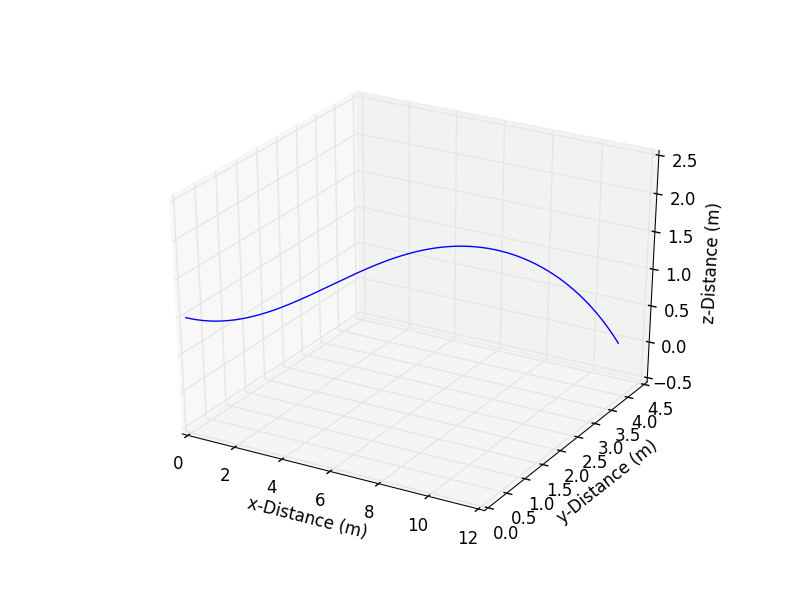
\includegraphics[width=16cm, height=10cm]{Simulated_throw_graph}
	\caption{3-dimensional representation of Frisbee trajectory produced under the following initial conditions: $v_x$=10.0 m/s, $v_y$=$v_z$=0.0 m/s, $\phi$=$\gamma$=0.0 radians, $\theta$=-0.25 radians, $\dot\phi$=$\dot\theta$=0.0 radians/s, and $\dot\gamma$=50.0 radians/s. Parameter values used to generate trajectory are shown in Table 2. }
\end{figure}

Since our data set did not have error bars, we arbitrarily assumed a constant error of 5 cm for each x, y, and z position in our synthetic trajectory. We created a text file containing a list of each time \textit{t}, a list of each x, y, and z position at time \textit{t}, and a list of error values for x(\textit{t}), y(\textit{t}), and z(\textit{t}). By removing certain timestamps from our simulated trajectory, it was possible to make the data either coarser or finer, in accordance with our overall goal. For example, pulling every 3rd timestamp (and corresponding position) from our data  allowed us to simulate camera footage captured at 100 FPS.

As described above, a coarse version of our simulated data set (100 FPS) was substituted for $\bold{X}$ in Equation 23. An array of parameters, $\theta$, was created such that the first four elements in the array were our unknowns ($P_{D0}, P_{D\alpha}, P_{L0}$, and $P_{L\alpha}$, and $P_{L0}$), and the remaining 6 elements were the true parameters used to generate the simulated data. $\bold{X}$ and $\theta$ as defined here were used to define Equation 24 in Python.

Finally, a Python package called "emcee" was used to perform MCMC analysis on our flying disc model. Four walkers were initialized in parameter space with Gaussian distribution around the parameter values we aimed to recover. (From H3, we expect that $P_{D0}, P_{D\alpha}, P_{L0}$, and $P_{L\alpha}$, and $P_{L0}$ take the values defined in Table 1.) A sampler in emcee was used to run MCMC for 20,000 steps, ultimately producing a chain of values for each parameter of interest.  This chain was used to generate a 4x4 corner plot illustrating the 2-d posterior probability distribution for each parameter. The mean value $\mu$ of each histogram along the diagonal of the 4x4 plot represented the maximum likelihood value of each parameter given our data set.

\subsection{FPS Effects}
After using MCMC analysis to whether we could recover the true lift and drag parameters used to simulate a Frisbee throw, we investigated the effects of increasingly coarse data sets on our ability to recover a single parameter ($P_{L0}$). From the original simulated data set, we created trajectories meant to replicate camera footage captured at 300 FPS, 150 FPS, 60 FPS, 30 FPS, 20 FPS, 12 FPS, 7.5 FPS, 6 FPS, 4 FPS, and 1 FPS.

For each dataset, MCMC analysis was performed to produce a posterior probability distribution for $P_{L0}$. The mean value of $P_{L0}$ was calculated for each FPS. The standard-deviation was also calculated for each camera speed. At lower FPS values, we expected larger standard deviations and less accurate recovery of the true parameter value for $P_{L0}$ (0.33).

\section{Results}

By generating a set of synthetic Frisbee flight coordinates and comparing the data to our model via Bayesian analysis, we assessed the ability of our model to recover the parameters used to simulate a thrown disc. Figure 5 depicts a 4x4 corner plot with the histograms along the diagonal showing the posterior probability distribution functions for our four lift and drag parameters. As indicated in Figure 5, the maximum likelihood values of each parameter given our synthetic data points were $P_{D0} = 0.18, P_{D\alpha}=0.69, P_{L0}=0.33$, and $P_{L\alpha}=1.9$. These recovered values aligned precisely with the actual values used to generate our simulated data set.


\begin{figure}[H]
        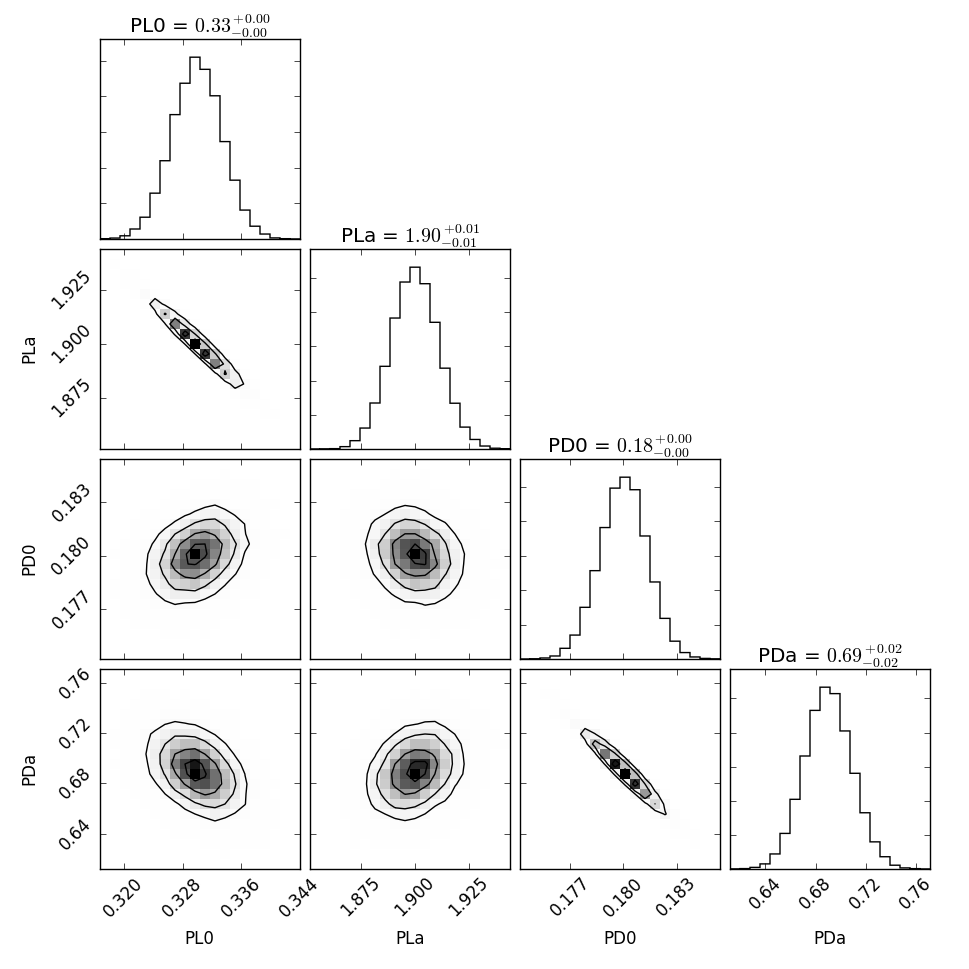
\includegraphics[width=12cm, height=12cm]{Final_PL0,PLa,PD0,PDa_nsteps=20,000_nwalkers=8}
	\centering
	\caption{Posterior probability distribution functions for lift and drag parameters. Numbers above each column indicate maximum likelihood value for $P_{D0}, P_{D\alpha}, P_{L0}$, and $P_{L\alpha}$, respectively. Non-diagonal histograms reflect correlation (or lack thereof) between individual parameters.}
\end{figure}
The non-diagonal plots depicted in Figure 5 yield information about the correlation between individual parameters. It indicates that $P_{D0}$ is inversely correlated with $P_{D\alpha}$, and that $P_{L0}$ is inversely correlated with $P_{L\alpha}$. That is, if we increase $P_{D\alpha}$ and $P_{L\alpha}$, $P_{D0}$ and $P_{L0}$ will decrease. These correlations agree with what we would expect, since both the lift and drag coefficients depend on their respective parameters only through $\alpha$, as reflected in Equations 3 and 4. In contrast, Figure 5 shows that there is no correlation between the lift and drag parameters. Again, we expect this result because the lift coefficient does not depend on the drag parameters, and likewise the drag coefficient does not depend on the lift parameters.

Figure 5 demonstrates that we can use Bayesian analysis to compare an experimental Frisbee trajectory to the one generated by our model under the same set of initial conditions. It further shows that, given a synthetic data set, such statistical analysis accurately recovers the known parameters used to simulate a thrown disc. Future work will compare model-generated data to experimental Frisbee trajectories presumably captured using video cameras.  Thus, going forward it will be highly important to understand the quality of the footage necessary to extract meaningful data.

To test the robustness of our Bayesian analysis given increasingly coarse data, we recorded the mean value of $P_{L0}$ for simulated Frisbee flights captured at 300, 150, 100, 600, 30, 20, 12, 7, 6, 4, and 3 FPS. As expected, at low FPS values, the recovered mean value of $P_{L0}$ varied significantly more around the true mean (0.33) than it did at high FPS values (Figure 6).
\begin{figure}[H]
        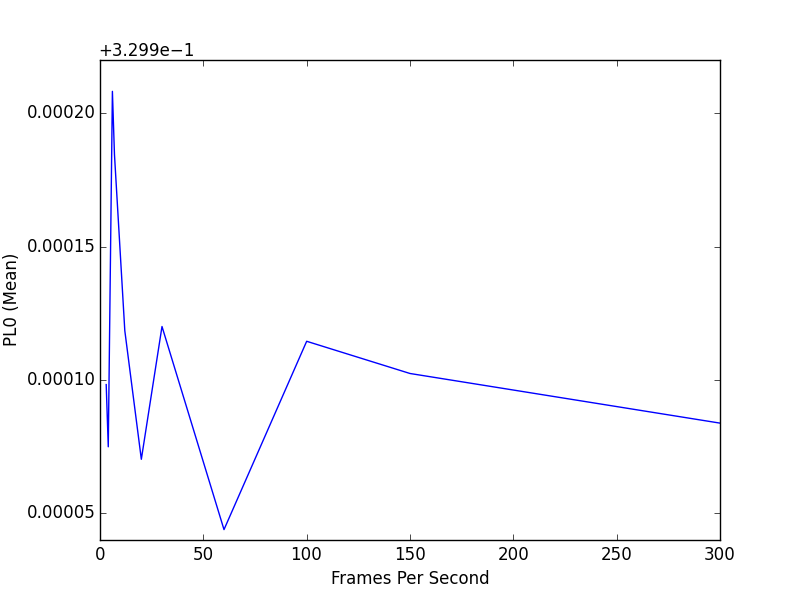
\includegraphics[width=10cm, height=6cm]{meanvsFPS}
	\centering
	\caption{Maximum likelihood value of $P_{L0}$ as a function of FPS. As FPS increases (indicating increasingly high video quality), the variance of $P_{L0}$ around 0.33 decreases.}
\end{figure}

We further quantified the effects of decreasing FPS on our ability to recover known Frisbee flight parameters by plotting $\mu/\sigma^2$ of our recovered $P_{L0}$ versus FPS for each FPS value (Figure 7). Again, as we would expect, this ratio decreases with increasing FPS due to decreasing $\sigma^2$ error. Around 250 FPS, the slope of $\mu/\sigma^2$ vs. FPS begins to level off, indicating that the $\sigma^2$ is remaining relatively stable around 0.001. 

\begin{figure}[H]
        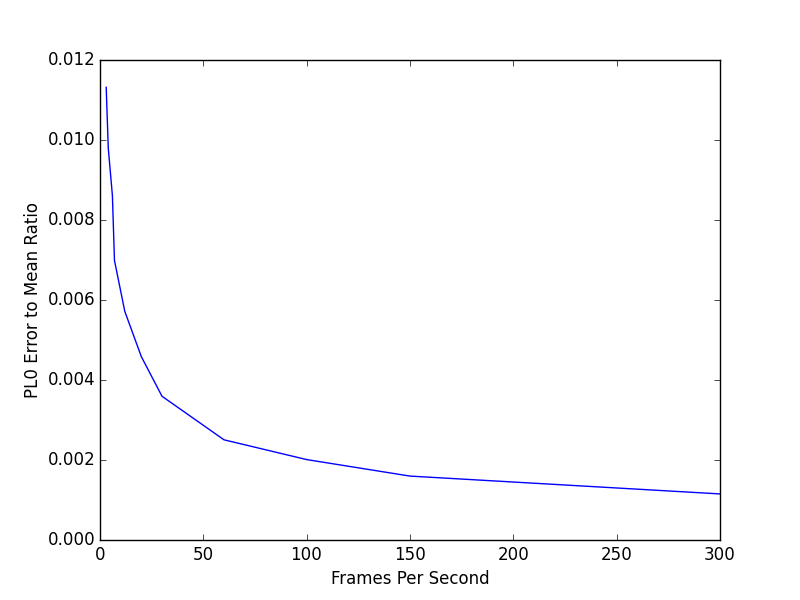
\includegraphics[width=10cm, height=6cm]{errortomeanratiovsFPS}
	\centering
	\caption{Value of $\mu$/$\sigma^2$ for $P_{L0}$ as a function of FPS. As FPS increases, $\mu$/$\sigma^2$ decreases at a decreasing rate.}
\end{figure}

Figures 6 and 7 suggest that a video camera that captures footage at a rate of 300 FPS may be sufficient to produce footage of flying discs that can be analyzed using the approach presented here. Expensive, high-speed cameras that capture at rates faster than 300 FPS are optimal for object tracking, but they may not be necessary to carry out our proposed parameter recovery method.

\section{Discussion}
The work presented here provides a method by which one can analyze the robustness of existing Frisbee models, and it offers an approach for assessing the reliability of video tracking methods that capture flight data.  Figure 4, which depicts successfully recovered parameter values from simulated flight data, suggests that an MCMC algorithm should be able to quantify the parameter values that generate actual data sets. By recovering parameter values from real data sets, inputting these values into our model, and comparing the corresponding model trajectory to actual flight data, future work can investigate whether the current Frisbee model yields realistic results. Moreover, where the model fails to match reality, future work can adjust it as necessary. 

Comparing a Frisbee model to real data, of course, wholly depends on one's ability to capture flight data at all. The two most widely used methods for capturing the motion of a Frisbee are 1) outfitting a disc with a gyroscope and an accelerometer, then tracking its flight and 2) recording a flying disc with a video camera, then applying video tracking software to determine its trajectory. Since instrumented discs may exhibit different physical properties than standard, non-instrumented discs, video tracking is likely a more reliable way to capture a Frisbee's motion without altering its trajectory. Figures 6 and 7 reflect a self-evident yet critically important fact: the error associated with video tracking methods increases with decreasing FPS. Thus, relatively high FPS equipment will be necessary to capture trajectories with enough timestamps to produce meaningful MCMC results. Future work should aim to quantify the lowest FPS value that will allow for successful parameter recovery. Since low-FPS cameras tend to be cheaper and more accessible than high-FPS cameras, it is in the best interest of researchers to identify an FPS threshold above which all results are equally meaningful. 

As disc sports grow in popularity, the science of flying discs must expand accordingly. In order for athletes to maximize their abilities, they must first understand the physical principles that govern their respective sports. By analyzing existing flying disc models and comparing their outputs to experimental flight data, future models can be fine-tuned such that they will be useful to athletes and coaches who hope to improve their on-field performances. The work presented here provides a springboard for achieving this level of refinement. We hope our analysis will help guide future Frisbee physicists in their endeavors.
\section{Acknowledgements}
This Honors Thesis would not have been possible without the generous, consistent, and enthusiastic support of Tom McClintock, whose help and mentorship are acknowledged with great appreciation. I am also especially grateful to Dr. Kevin Lin for his advice and guidance, and for his continued support of my academic pursuits. Finally, thank you to the incredible Tucson Ultimate community, which helped me realize that flying discs are not just for dogs.

\bibliography{ThesisRefs}
\bibliographystyle{plain}

\end{document}  
